
%usepackage es egyebek
\pdfminorversion=4
\documentclass[17pt]{extarticle}

\usepackage[margin=1.5cm,nohead]{geometry}
\usepackage[utf8]{inputenc}
\usepackage[hungarian]{babel}


\usepackage[%hypertex,
   unicode=true,
   plainpages = false,
   pdfpagelabels,
   bookmarks=true,
   bookmarksnumbered=true,
   bookmarksopen=true,
   breaklinks=true,
   backref=false,
   colorlinks=true,
   linkcolor = blue,
   urlcolor  = blue,
   citecolor = red,
   anchorcolor = green,
   hyperindex = true,
   hyperfigures,
%   pdftex
]{hyperref}
\hypersetup{
   pdftitle={Feladatok},
   pdfauthor={Czylabson Asa},
   pdfsubject={Hold Föld Nap},
}


\usepackage{amsmath}
\usepackage{amsfonts}
\usepackage{amssymb}
\usepackage{graphicx}
\usepackage{type1cm}
\usepackage{setspace}
\usepackage{mathtools}


%\usepackage{xcolor}
%\usepackage{tikz,lipsum,lmodern}
\usepackage[most]{tcolorbox}


\usepackage{matlab-prettifier}
\usepackage[T1]{fontenc}
\usepackage{listingsutf8}

\lstset{
   style              = Matlab-editor,
   basicstyle         = \mlttfamily,
   escapechar         = ",
   mlshowsectionrules = true,
   literate= {á}{{\'{a}}}1 {Á}{{\'{A}}}1 {é}{{\'{e}}}1 {É}{{\'{E}}}1 {í}{{\'{i}}}1 {Í}{{\'{I}}}1 {ó}{{\'{o}}}1 {Ó}{{\'{O}}}1  {ö}{{\"{o}}}1 {Ö}{{\"{O}}}1 {ő}{{\H{o}}}1 {Ő}{{\H{O}}}1 {ú}{{\'{u}}}1 {Ú}{{\'{U}}}1  {ü}{{\"{u}}}1 {Ü}{{\"{U}}}1 {ű}{{\H{u}}}1 {Ű}{{\H{U}}}1
}


%zarojel, FA...
% ez valahol kellett
\DeclarePairedDelimiter\ceil{\lceil}{\rceil}
\DeclarePairedDelimiter\floor{\lfloor}{\rfloor}

% zárójelek stb.
\newcommand{\Gzjel}[1]{%
{ \left( #1 \right) }
}

\newcommand{\gzjel}[1]{%
{ \left( #1 \right) }
}

\newcommand{\Toligv}[2]{%
#1,\hdots ,#2
}

\newcommand{\GZJ}[1]{%
{ \left( #1 \right) }
}

\newcommand{\KZJ}[1]{%
{ \{ #1 \} }
}

\newcommand{\szzjel}[1]{%
{ \left[ #1 \right] }
}

\newcommand{\Tolig}[2]{%
#1\hdots #2
}

\newcommand{\SZOR}[2]{%
#1\cdot\hdots\cdot #2
}

% integrál rendes d-vel
\newcommand{\mint}[2]{%
\int #1 \text{d}#2
}

\newcommand{\mder}[2]{%
\frac{\text{d} #1}{\text{d}#2}
}


% ez máshogy van alapban
\newcommand{\tg}[0]{%
\tan
}

\newcommand{\ctg}[0]{%
\cot
}

\newcommand{\D}[1]{%
{{\mathbb{D}\szzjel{#1}}}
}

\newcommand{\V}[1]{%
{{{\mathbb{D}}^{2}\szzjel{#1}}}
}


\newcommand{\E}[1]{%
{{\mathbb{E}\szzjel{#1}}}
}

\newcommand{\A}[1]{%
{\mathbb{A}\szzjel{#1}}
}

\newcommand{\hehu}[1]{%
\hspace{0.5cm}#1\hspace{0.5cm}
}






% rövidítések
% rövid alakok a hosszabb szavakra
\newcommand{\fv}[1]{%
függvény#1
}

\newcommand{\Fv}[1]{%
Függvény#1
}

\newcommand{\der}[1]{%
derivált#1
}

\newcommand{\Der}[1]{%
Derivált#1
}

\newcommand{\de}[1]{%
differenciálegyenlet#1
}

\newcommand{\De}[1]{%
Differenciálegyenlet#1
}

\newcommand{\kef}[1]{%
kezdeti érték feladat#1
}

\newcommand{\Kef}[1]{%
Kezdeti érték feladat#1
}


\newcommand{\amgm}[1]{%
számtani-mértani közép#1
}
\newcommand{\Amgm}[1]{%
Számtani-mértani közép#1
}
\newcommand{\gmhm}[1]{%
mértani-harmonikus közép#1
}
\newcommand{\Gmhm}[1]{%
Mértani-harmonikus közép#1
}

\newcommand{\amqm}[1]{%
számtani-négyzetes közép#1
}
\newcommand{\Amqm}[1]{%
Számtani-négyzetes közép#1
}


\newcommand{\szigmon}[1]{%
szigorúan monoton#1
}
\newcommand{\Szigmon}[1]{%
Szigorúan monoton#1
}
\newcommand{\nov}[1]{%
növekvő#1
}
\newcommand{\Nov}[1]{%
Növekvő#1
}

\newcommand{\elen}[1]{%
egyenlőtlenség#1
}

\newcommand{\Elen}[1]{%
Egyenlőtlenség#1
}

\newcommand{\vv}[1]{%
valségi változó#1
}

\newcommand{\Vv}[1]{%
Valségi változó#1
}

\newcommand{\leb}[0]{%
lebegőpontos
}

\newcommand{\Leb}[0]{%
Lebegőpontos
}





% tcolorbox-al kapcsolatos
\newcommand{\feher}[1]{%
\begin{tcolorbox}[colback=white]
#1
\end{tcolorbox}
}

\newcommand{\zold}[1]{%
\begin{tcolorbox}[colback=green!17]
#1
\end{tcolorbox}
}

\newcommand{\szurke}[1]{%
\begin{tcolorbox}[colback=gray!10!white]
#1
\end{tcolorbox}
}

\newcommand{\szurkeM}[1]{%
\begin{tcolorbox}[colback=gray!10!white, top=-5mm, bottom=3mm]
\begin{gather*}
#1
\end{gather*}
\end{tcolorbox}
}


\newcommand{\sarga}[1]{%
\begin{tcolorbox}[colback=yellow!10!white]
#1
\end{tcolorbox}
}

\newcommand{\barna}[1]{%
\begin{tcolorbox}[colback=brown!20!white]
#1
\end{tcolorbox}
}

\newcommand{\kek}[1]{%
\begin{tcolorbox}[colback=blue!20!white]
#1
\end{tcolorbox}
}

\newcommand{\Fa}[1]{%
\begin{tcolorbox}[colback=brown!20!white]
#1
\end{tcolorbox}
}

\newcommand{\Fnew}[0]{%
\end{tcolorbox}
\begin{tcolorbox}[colback=brown!20!white]
}




\newcommand{\Mo}[1]{%
\begin{tcolorbox}[colback=green!17]
#1
\end{tcolorbox}
}


\newcommand{\Mnew}[0]{%
\end{tcolorbox}
\begin{tcolorbox}[colback=green!17]
}


\newcommand{\egy}[1]{%
\Fa{\input{#1Fa}}
\Mo{\input{#1Mo}}
}


\definecolor{light-gray}{gray}{0.95}
\newcommand{\mcode}[1]{
   \colorbox{light-gray}{\texttt{#1}}
}


\begin{document}\begin{spacing}{1.2}

\section*{Nevezetes határértékek} \label{DB}
\nameref{DBe}
\newline
\nameref{DBnthroot}
\newpage
\section*{az e-szám} \label{DBe}
\nameref{DBe1}
\vspace{0.5cm}
\LINK{
\hfill\nameref{DB}
}
\newpage
\section*{alap-Fa} \label{DBe1}
\Fa{
\Mat{
   \exists \lim_{n\to \infty} \gzjel{ 1+\frac{1}{n}}^{n}
}

}
\vspace{0.5cm}
\LINK{
\nameref{DBe1Mo}
\hfill\nameref{DBe}
}
\newpage
\section*{alap-Mo} \label{DBe1Mo}
\Mo{
A \amgm{}miatt:
\Mat{
   1\gzjel{ 1+\frac{1}{n}}^{n}<
   \gzjel{\frac{1 + 1+\frac{1}{n}+\cdots+1+\frac{1}{n}}{n+1}}^{n+1}=
   \gzjel{ 1+\frac{1}{n+1}}^{n+1}
}
az $a_n=\gzjel{1+\frac{1}{n}}^{n}$ \szigmon{}nő.


A \gmhm{}miatt:
\Mat{
   1\gzjel{ 1+\frac{1}{n}}^{n+1}>
   \gzjel{\frac{n+2}{1 + 1-\frac{1}{n+1}+\cdots+1-\frac{1}{n+1}}}^{n+2}=\\
   =\gzjel{ 1+\frac{1}{n+1}}^{n+2}
}
az $b_n=\gzjel{1+\frac{1}{n}}^{n+1}$ \szigmon{}csökken.
Könnyen látható, hogy:
\Mat{
   a_n < b_m \hspace{1cm} \forall m,n \\
   b_n-a_n=\frac{a_n}{n}
}
Mindezek miatt a sorozatok konvergensek és a határértékeik egybeesnek. Ezt
a számot e-vel szokták jelölni.

}
\vspace{0.5cm}
\LINK{
\nameref{DBe1}
\hfill\nameref{DBe}
}
\newpage
\section*{n-edik gyök} \label{DBnthroot}
\nameref{DBnthrootSum}
\newline
\nameref{DBnthroot1}
\newline
\nameref{DBnthroot2}
\newline
\nameref{DBnthroot2a}
\newline
\nameref{DBnthroot3}
\vspace{0.5cm}
\LINK{
\hfill\nameref{DB}
}
\newpage
\section*{Létezés...-Fa} \label{DBnthrootSum}
\Fa{
\szurkeM{
   a,b\in \mathbb{R}, \ n\in\mathbb{N}\\
   \forall \ a>0, n>1 \ : \ \exists! \ b>0 \ : \ b^n=a \\
   \text{jele:}\ b=a^{\frac{1}{n}}
}
Tulajdonság:
\szurkeM{
   (a^{\frac{1}{n}})^m=(a^m)^\frac{1}{n}
}

}
\vspace{0.5cm}
\LINK{
\nameref{DBnthrootSumMo}
\hfill\nameref{DBnthroot}
}
\newpage
\section*{Létezés...-Mo} \label{DBnthrootSumMo}
\Mo{
Legyen $a>1$ és
\szurkeM{
   a_{-}=\{ b\ :\ b^n < a \}\\
   a_{+}=\{ b\ :\ b^n > a \}
}
Megfigyelések:
\begin{itemize}
   \item $a_{-}$ és $a_{+}$ nemüresek
   \item bármely $b\in a_{+}$ felső korlátja $a_{-}$
   \item bármely $b\in a_{-}$ alsó korlátja $a_{+}$
\end{itemize}
A valós számok felső/alsó-határ tulajdonsága miatt egyértelműen létezik
$S=\sup a_{-}$ és $I=\inf a_{+}$ és $S\le I.$
Ha $S < I$ akkor az ábra segít megtalálni az ellentmondást:
\begin{center}
\frame{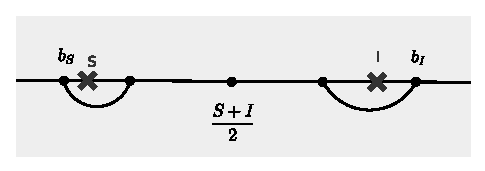
\includegraphics[scale=1.2]{DB/fig/nthroot}}
\end{center}
Tehát $S=I.$ Ezért: $I^n = S^n \le a$ és $I^n\ge a$, vagyis az $S=I$ szám
valóban $a^{\frac{1}{n}}$-ként viselkedik.
%!TODO!


}
\vspace{0.5cm}
\LINK{
\nameref{DBnthrootSum}
\hfill\nameref{DBnthroot}
}
\newpage
\section*{konstans-Fa} \label{DBnthroot1}
\Fa{
\szurkeM{
   a^{\frac{1}{n}} \to 1 \hspace{1cm} a\in\mathbb{R}
}

}
\vspace{0.5cm}
\LINK{
\nameref{DBnthroot1Mo}
\hfill\nameref{DBnthroot}
}
\newpage
\section*{konstans-Mo} \label{DBnthroot1Mo}
\Mo{
Legyen $a>1$, ekkor valamely $a_n>0$ sorozattal $a^{\frac{1}{n}}=1+a_n$.
A következő megállapításokat tehetjük:
\szurkeM{
   a=\gzjel{1+a_n}^n \ge 1+na_n \hspace{1cm}(\text{Bernoulli})\\
   \frac{a-1}{n}\ge a_n \\
   1\le a^{\frac{1}{n}}\le 1+\frac{a-1}{n}\hspace{1cm}(\text{rendőr-elv})
}
$a<1$ esetén alkalmazzuk $\frac{1}{a}$-ra a fentieket.

}
\vspace{0.5cm}
\LINK{
\nameref{DBnthroot1}
\hfill\nameref{DBnthroot}
}
\newpage
\section*{$n$-Fa} \label{DBnthroot2}
\Fa{
\szurkeM{
   n^{\frac{1}{n}} \to 1
}

}
\vspace{0.5cm}
\LINK{
\nameref{DBnthroot2Mo}
\hfill\nameref{DBnthroot}
}
\newpage
\section*{$n$-Mo} \label{DBnthroot2Mo}
\Mo{
A következő megállapításokat tehetjük:
\szurkeM{
   n=\gzjel{1+a_n}^n \ge 1+\frac{n(n-1)}{2}a^2_n \hspace{1cm}(\text{Binomiális})\\
   \sqrt{\frac{2}{n}}\ge a_n \\
   1\le n^{\frac{1}{n}}\le 1+\sqrt{\frac{2}{n}}\hspace{1cm}(\text{rendőr-elv})
}

}
\vspace{0.5cm}
\LINK{
\nameref{DBnthroot2}
\hfill\nameref{DBnthroot}
}
\newpage
\section*{polinom-Fa} \label{DBnthroot2a}
\Fa{
\szurkeM{
   a_0,\hdots,a_m>0\\
   P(n)=\sum_{k=0}^m a_k n^k \\
   P(n)^{\frac{1}{n}}\to 1
}

}
\vspace{0.5cm}
\LINK{
\nameref{DBnthroot2aMo}
\hfill\nameref{DBnthroot}
}
\newpage
\section*{polinom-Mo} \label{DBnthroot2aMo}
\Mo{
Legyen $a=\max\{ a_0,\hdots,a_m \}$:
\szurkeM{
   a_m n^m \le P(n) \le (m+1)an^m \hspace{1cm} (\text{rendőr-elv})
}

}
\vspace{0.5cm}
\LINK{
\nameref{DBnthroot2a}
\hfill\nameref{DBnthroot}
}
\newpage
\section*{$n!$-Fa} \label{DBnthroot3}
\Fa{
\szurkeM{
   (n!)^{\frac{1}{n}} \to \infty
}

}
\vspace{0.5cm}
\LINK{
\nameref{DBnthroot3Mo}
\hfill\nameref{DBnthroot}
}
\newpage
\section*{$n!$-Mo} \label{DBnthroot3Mo}
\Mo{
A \amqm{}és egyszerű átalakítás mutatja:
\szurkeM{
   \gzjel{\frac{\sum{\frac{1}{k}}}{n}}^2\le
   \frac{\sum{\frac{1}{k^2}}}{n}\le
   \frac{\sum{\frac{2}{k(k+1)}}}{n}=
   2\frac{1-\frac{1}{n+1}}{n}\le\frac{2}{n}
}
A \gmhm{ből:}
\szurkeM{
   (n!)^{\frac{1}{n}} \ge \frac{n}{\sum\frac{1}{k}}\ge
   \sqrt{\frac{n}{2}}
}

}
\vspace{0.5cm}
\LINK{
\nameref{DBnthroot3}
\hfill\nameref{DBnthroot}
}
\newpage

\end{spacing}
\end{document}

